\chapter{Unified Process (UP)}

\section{OOA e OOD}

\dfn{OOA/D}{
    \begin{itemize}
        \item [$\Rightarrow$] \textbf{OOA} (Object Oriented Analysis): studio dei requisiti e delle specifiche del sistema;
        \item [$\Rightarrow$] \textbf{OOD} (Object Oriented Design): progettazione del sistema.
    \end{itemize}

    Per studiare OOA/D si utilizza Unified Process, 
    un processo di sviluppo software orientato agli oggetti.
}

\nt{UP può essere applicato usando un 
approccio agile come Scrum o XP.}

\cor{UML}{
    UP utilizza UML come linguaggio di modellazione.
    UML è un linguaggio di modellazione grafico e testuale
    per la specifica, la costruzione e la documentazione
    di sistemi software orientati agli oggetti.

}

\wc{UML descrive il software}{ UML non è nato per descrivere software, ma
per descrivere \fancyglitter{concetti}\footnote{Simile a ER, visto nel corso "Basi di dati".}.}

\subsubsection{OOD è guidata dalle responsabilità (si vedano
i pattern GRASP):}

\begin{itemize}
    \item [$\Rightarrow$] Quali sono gli oggetti? Quali sono le classi?
    \item [$\Rightarrow$] Cosa deve conoscere un oggetto? Cosa deve saper fare?
    \item [$\Rightarrow$] Come collaborano gli oggetti?
\end{itemize}

\dfn{Pattern}{
    I pattern sono euristiche, best practice, che aiutano a codificare principi
    di soluzioni.
}


\subsubsection{ODD è correlata all'analisi dei requisiti:}

\begin{itemize}
    \item [$\Rightarrow$] \fancyglitter{Casi d'uso};
    \item [$\Rightarrow$] \fancyglitter{Storie utente}.
\end{itemize}

\ex{Gioca una \newfancyglitter{partita a dadi}}{
\subsubsection{Definizione dei casi d'uso: storie scritte.}

Il \newfancyglitter{Giocatore} chiede
di \fancyglitter{lanciare} i \newfancyglitter{dadi}. Il Sistema presenta il
\fancyglitter{risultato}: se \fancyglitter{il valore totale} delle facce dei dadi
è sette, il giocatore ha vinto; altrimenti ha
perso.

\subsubsection{Definizione di un modello di dominio:
\newfancyglitter{i concetti o gli oggetti significativi}.}

\begin{center}
    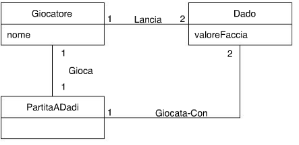
\includegraphics[scale=0.7]{images/Dadi.png}
\end{center}

\subsubsection{Assegnare responsabilità agli oggetti e 
disegnare diagrammi di interazione: \fancyglitter{responsabilità e collaborazioni}.}

\begin{center}
    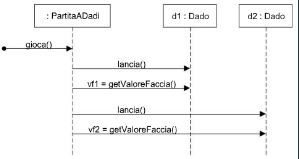
\includegraphics[scale = 0.7]{images/Dadi2.png}
\end{center}

\subsubsection{Definizione dei diagrammi delle classi di progetto.}

\begin{center}
    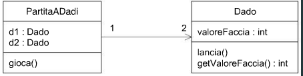
\includegraphics[scale=0.7]{images/Dadi 3.png}
\end{center}

}
\subsubsection{}
L'analisi dei requisiti e l'OOA/D vanno svolte nel contesto di un processo di sviluppo:

\begin{itemize}
    \item [$\Rightarrow$] Sviluppo iterativo;
    \item [$\Rightarrow$] Approccio agile;
    \item [$\Rightarrow$] Unified Process (UP).
\end{itemize}

\nt{ER e UML non sono pienamente adatti a possibili incrementi.}
\pagebreak

\subsection{UML}

\dfn{UML}{UML è un linguaggio \newfancyglitter{visuale} per la specifica,
la costruzione e la documentazione degli elaborati di un sistema software.

UML è uno standard per la notazione di diagrammi per disegnare o rappresentare
figure relative al software (specialmente OO).}
\subsubsection{}
UML è un \textit{abbozzo} o un \textit{progetto} per aiutare la comprensione nei team di sviluppo.
Il termine abbozzo indica che può essere soggetto a correzione, ma se non ci 
sono feedback a tal proposito deve essere trattato come un dizionario.

\subsubsection{Uso di UML:}

\begin{itemize}
    \item [$\Rightarrow$] Punto di vista \fancyglitter{concettuale}: modello 
    di dominio, per visualizzare concetti del mondo reale;
    \item [$\Rightarrow$] Punto di vista \fancyglitter{software}: diagramma
    delle classi di progetto, utilizzata per visualizzare elementi software.
\end{itemize}

\subsubsection{Brevi note storiche:}

\begin{itemize}
    \item [$\Rightarrow$] Anni '60 e '70: nascita dei linguaggi OO (Simula e Smalltalk);
    \item [$\Rightarrow$] 1988: Bertrand Meyer, "Object-Oriented Software";
    \item [$\Rightarrow$] 1991: Jim Rumbaugh, "Object-Oriented Modelling and Design" (OOA/D);
    \item [$\Rightarrow$] 1991, Grady Booch, "Object-Oriented Software Engineering" (OOA/D e Casi d'Uso);
    \item [$\Rightarrow$] 1994, Rumbaugh e Booch fanno le prime proposte di UML;
    \item [$\Rightarrow$] Rational Corporation fondata dai "tre amigos" (Jacobson, Booch e Rumbaugh);
    \item [$\Rightarrow$] 1997 UML 1;
    \item [$\Rightarrow$] 2004 UML 2 (usato attualmente).
\end{itemize}

\section{Unified Process}

\dfn{Unified Process}{
    Unified Process è un processo iterativo ed evolutivo (incrementale)
    per lo sviluppo del software per la costruzione di sistemi orientati agli oggetti.
    Le iterazioni iniziali sono guidate dal \newfancyglitter{rischio}, dal
    \newfancyglitter{cliente} e dall'\newfancyglitter{architettura}.
}

\qs{}{Cosa c'è in UP?}

\begin{itemize}
    \item [$\Rightarrow$] Un'organizzazione del piano di progetto
    per fasi sequenziali;
    \item [$\Rightarrow$] Indicazioni sulle attività da svolgere nell'ambito
    di discipline e sulle loro inter-relazioni;
    \item [$\Rightarrow$] Un insieme di ruoli predefiniti;
    \item [$\Rightarrow$] Un insieme di artefatti da produrre.
\end{itemize}

\subsubsection{Un progetto UP è organizzato in 4 fasi:}

\begin{itemize}
    \item [$\Rightarrow$] \fancyglitter{Ideazione} (inception): visione approssimativa, studio economico, portata, stime approssimative di costi e tempi. \textbf{\underline{Milestone}:} \newfancyglitter{Obiettivi};
    \item [$\Rightarrow$] \fancyglitter{Elaborazione} (elaboration): visione raffinata, è un'implementazione iterativa del nucleo dell'architettura, risoluzione dei rischi maggiori, identificazione della maggior parte dei requisiti e della portata, stime più realistiche sulle loro inter-relazioni. \textbf{\underline{Milestone}:} \newfancyglitter{Architetturale};  
    \item [$\Rightarrow$] \fancyglitter{Costruzione} (construction): implementazione iterativa degli elementi rimanenti, più facili e a rischio minore, preparazione al rilascio. \textbf{\underline{Milestone}:} \newfancyglitter{Capacità operazionale};
    \item [$\Rightarrow$] \fancyglitter{Transizione} (transition): beta test, rilascio. \textbf{\underline{Milestone}:} \newfancyglitter{Rilascio prodotto}.
\end{itemize}

\begin{center}
    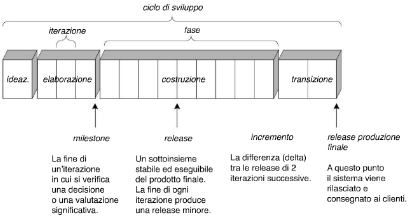
\includegraphics[scale = 1]{images/UP.png}
\end{center}

\wc{L'ideazione e l'elaborazione sono fasi di requisiti}{
    \begin{itemize}
        \item [$\Rightarrow$] L'Ideazione non è una fase di requisiti, ma di fattibilità;
        \item [$\Rightarrow$] L'Elaborazione non è una fase di requisiti o di progettazione, ma una fase in cui 
        si implementa in modo iterativo l'architettura del sistema e vengono ridotti i rischi maggiori.
    \end{itemize}
}

\subsection{Le discipline}

\dfn{Discipline}{
    Una disciplina è un insieme di attività e dei relativi \newfancyglitter{elaborati}
    in una determinata area, come le attività relative all'analisi dei requisiti. 
}

\cor{Elaborato}{
    Un elaborato (artefatto o work product) è il termine generico che indica un qualsiasi prodotto di lavoro: codice, schemi di basi di dati, 
    documenti di testo, diagrammi, modelli, etc.
}

\subsubsection{Discipline ingegneristiche di UP:}

\begin{itemize}
    \item [$\Rightarrow$] \fancyglitter{Modellazione del business}: attività che 
    modellano il dominio del problema e il suo ambito;
    \item [$\Rightarrow$] \fancyglitter{Requisiti}: attività di raccolta dei requisiti;
    \item [$\Rightarrow$] \fancyglitter{Progettazione} (analysis and design): attività di analisi dei requisiti
    e progetto architetturale;
    \item [$\Rightarrow$] \fancyglitter{Implementazione}: attività di progetto dettagliato e codifica del sistema, test sui componenti;
    \item [$\Rightarrow$] \fancyglitter{Test}: attività di controllo di qualità, test di integrazione e di sistema;
    \item [$\Rightarrow$] \fancyglitter{Rilascio}: attività di consegna e messa in opera.
\end{itemize}

\subsubsection{Discipline di supporto di UP:}

\begin{itemize}
    \item [$\Rightarrow$] \fancyglitter{Gestione delle configurazioni e del cambiamento}: attività di manutenzione durante il progetto;
    \item [$\Rightarrow$] \fancyglitter{Gestione progetto}: attività di pianificazione e governo del progetto;
    \item [$\Rightarrow$] \fancyglitter{Infrastruttura} (enviroment): attività che supportano il team di progetto, riguardo ai processi e strumenti utilizzati.
\end{itemize}

\nt{Nonostante le fasi siano \newfancyglitter{sequenziali}, le discipline non lo sono (perchè si eseguono in ogni iterazione).
Il numero di iterazioni dipende dal Project Manager.}

\subsubsection{Uso di UML in UP:}

\begin{itemize}
    \item [$\Rightarrow$] UP usa solo UML come linguaggio di modellazione;
    \item [$\Rightarrow$] I diagrammi UML si usano con variabilità, bisogna \newfancyglitter{personalizzare} UP;
    \item [$\Rightarrow$] I diagrammi si usano in UP seguendo le iterazioni e gli incrementi;
    \item [$\Rightarrow$] UP dice \newfancyglitter{quando} usare un diagramma;
    \item [$\Rightarrow$] In UP quasi tutto è \newfancyglitter{opzionale} eccetto che lo sviluppo iterativo e guidato dal rischio, la verifica continua della qualità e il codice;
    \item [$\Rightarrow$] La scelta delle pratiche e degli artefatti UP si riassume in un documento (\newfancyglitter{scenario di sviluppo}).
\end{itemize}

\subsection{Che cosa sono i requisiti?}

\dfn{Requisito}{
    Un requisito è una \newfancyglitter{capacità} o una condizione a cui il sistema deve essere \newfancyglitter{conforme}.
}

\cor{Sorgenti dei requisiti}{
    I requisiti derivano da richieste degli utenti del sistema per risolvere dei problemi e raggiungere degli obiettivi.
    Possono essere:
    \begin{itemize}
        \item [$\Rightarrow$] \fancyglitter{Requisiti funzionali}: descrivono il comportamento del sistema in termini di funzionalità offerte;
        \item [$\Rightarrow$] \fancyglitter{Requisiti non funzionali}: le proprietà del sistema nel suo complesso (sicurezza, prestazioni, etc.).
    \end{itemize}
}

\clm{}{}{
    In UP bisogna gestire i requisiti: si utilizza un approccio sistematico
    per trovare, documentare, organizza e tracciare i \underline{requisiti che cambiano}
    di un sistema. Si inizia a programmare quando sono stati specificati il 10\% o il 20\%
    dei requisiti significativi.
}

\subsubsection{Acquisizione sistematica dei requisiti:}

\begin{itemize}
    \item [$\Rightarrow$] Scrivere i Casi d'Uso con i clienti;
    \item [$\Rightarrow$] Workshop dei requisiti con sviluppatori e clienti;
    \item [$\Rightarrow$] Gruppi di lavoro con rappresentanti dei clienti;
    \item [$\Rightarrow$] Dimostrazione ai clienti dei risultati di ciascuna iterazione, per favorire un feedback.
\end{itemize}

\subsubsection{Modello FURPS+:}

\begin{itemize}
    \item [$\Rightarrow$] \fancyglitter{Funzionali} (F): requisiti funzionali e di sicurezza;
    \item [$\Rightarrow$] \fancyglitter{Usabilità} (U): facilità d'uso del sistema;
    \item [$\Rightarrow$] \fancyglitter{Affidabilità} (R - Reliability): disponibilità del sistema, capacità di tollerare guasti o di essere ripristinato;
    \item [$\Rightarrow$] \fancyglitter{Prestazioni} (P): tempi di risposta, throughput, capacità e uso delle risorse;
    \item [$\Rightarrow$] \fancyglitter{Sostenibilità} (S): facilità di modifica per riparazioni e miglioramenti, adattabilità, manutenibilità, localizzazione, configurazione, compatibilità;
    \item [$\Rightarrow$] \fancyglitter{+}: vincoli di progetto, interoperabilità, operazionali, fisici, legali, etc.
\end{itemize}

\subsubsection{Elaborati:}

\begin{itemize}
    \item [$\Rightarrow$] \fancyglitter{Modello dei Casi d'Uso}: scenari tipi dell'utilizzo di un sistema;
    \item [$\Rightarrow$] \fancyglitter{Specifiche supplementari}: ciò che non rientra nei Casi d'Uso, requisiti non funzionali o funzionali non esprimibili attraverso i Casi d'Uso;
    \item [$\Rightarrow$] \fancyglitter{Glossario}: termini significativi, dizionario dei dati;
    \item [$\Rightarrow$] \fancyglitter{Visione}: riassume i requisiti di alto livello, un documento sintetico per apprendere rapidamente le idee principali del progetto;
    \item [$\Rightarrow$] \fancyglitter{Regole di Business}: regole di dominio, i requisiti o le politiche che trascendono un unico progetto software e a cui un sistema deve conformarsi.
\end{itemize}

\section{Ideazione}

\qs{}{Che cos'è l'ideazione?}

\paragraph{Risposta:} l'ideazione permette di stabilire una visione completa
e la portata del progetto (\newfancyglitter{studio di fattibilità}).

\subsubsection{Durante l'ideazione:}

\begin{itemize}
    \item [$\Rightarrow$] Si analizzano il 10\% dei Casi d'Uso;
    \item [$\Rightarrow$] Si analizzano i requisiti non funzionali più importanti;
    \item [$\Rightarrow$] Si realizza una stima dei costi;
    \item [$\Rightarrow$] Si prepara l'ambiente di sviluppo;
    \item [$\Rightarrow$] \newfancyglitter{Durata:} breve.
\end{itemize}

\clm{}{}{Lo scopo dell'Ideazione \underline{non} è di raccogliere tutti i requisiti, né di generare
una stima o un piano di progetto affidabile.
Durante l'ideazione si cerca di capire se il progetto è fattibile e se ha senso.}

\definecolor{dkgreen}{rgb}{0, 0.5, 0}
\definecolor{mgray}{rgb}{0.9, 0.9, 0.9}
\begin{center}
    \begin{tabular}{ || >{\columncolor{mgray}}p{8cm} | >{\columncolor{GreenPastel}}p{8cm} ||}
    \hline\hline
        \rowcolor{lightgray}
    \textbf{Elaborato}& \textbf{\textcolor{dkgreen}{Commento}}\\ \hline
    \hline
        Visione e studio economico & Descrive obiettivi e vincoli di alto livello, fornisce un sommario del progetto.\\ \hline

        Modello dei Casi d'Uso & Descrive i requisiti funzionali del sistema. Vengono identificati i nomi della maggior parte dei Casi d'Uso.\\ \hline

        Specifiche supplementari & Descrive i requisiti non funzionali e i requisiti funzionali non esprimibili attraverso i Casi d'Uso.\\ \hline

        Glossario & Definisce i termini significativi del dominio.\\ \hline

        Lista dei Rischi e Piano di Gestione dei Rischi & Identifica i rischi principali e come affrontarli.\\ \hline

        Prototipi e proof of concept & Dimostrano la fattibilità tecnica e la comprensione dei requisiti.\\ \hline

        Piano dell'Iterazione & Fornisce una descrizione di cosa fare nella prima iterazione dell'elaborazione.\\ \hline

        Piano delle Fasi e Piano di Sviluppo del Software & Ipotesi (poco precise) riguardo la fase di elaborazione.\\ \hline 
    
        Scenario di Sviluppo & Descrive le pratiche e gli artefatti UP da usare.\\ \hline
    
        \hline

    \end{tabular}
\end{center}

\subsection{Artefatti nell'Ideazione}

\qs{}{La documentazione non è troppa?}

\paragraph{Risposta:} lo scopo della documentazione non è nel documento in sè, ma nel pensare:

\begin{itemize}
    \item [$\Rightarrow$] gli artefatti sono quelli che aggiungono valore;
    \item [$\Rightarrow$] sono parzialmente completati;
    \item [$\Rightarrow$] sono preliminari e approssimativi.
\end{itemize}

\nt{Nessun documento è definitivo.}

\dfn{Specifiche supplementari}{
    Le \newfancyglitter{specifiche supplementari} raccolgono altri requisiti,
    informazioni e vincoli che non sono espressi nei Casi d'Uso o nel Glossario. 
    Si deve mettere anche la cronologia delle versioni.
}

\subsection{Tipologie di documenti}

\dfn{Visione}{
    Il documento \newfancyglitter{Visione} riassume alcune informazioni contenute nel modello dei Casi d'Uso e 
    nelle Specifiche supplementari. Inoltre descrive brevemente il progetto ai partecipanti per stabilire una
    visione comune.
    
    \begin{itemize}
        \item [$\Rightarrow$] Obiettivi e problemi fondamentali ad alto livello\footnote{Soprattutto per i requisiti non funzionali};
        \item [$\Rightarrow$] Riepilogo delle caratteristiche di sistema.
    \end{itemize}
}

\nt{Spesso è utile iniziare da un Glossario.}

\dfn{Glossario e dizionario dei dati}{
    Il \newfancyglitter{Glossario} è un documento che definisce i termini significativi del dominio e le relazioni tra di
    essi. Si devono eliminare eventuali discrepanze per ridurre problemi di comunicazione e di ambiguità.

    In UP il Glossario svolge anche il ruolo di \newfancyglitter{dizionario dei dati}:
    un documento di dati che si riferiscono ad altri dati\footnote{Metadati.}, per esempio le regole di validazione.
}

\cor{Regole di dominio}{
    Le \newfancyglitter{regole di dominio} (o regole di Business\footnote{Viste in "Basi di dati".}) stabiliscono
    come può funzionare un dominio o un business.

}


\section{Casi d'Uso}

\subsection{Disciplina dei requisiti}

\dfn{Disciplina dei requisiti}{
    La \newfancyglitter{disciplina dei requisiti} è il processo
    per scoprire cosa deve essere costruito e orientare lo sviluppo verso 
    il sistema corretto.
}

\cor{Requisiti di sistema}{
    I requisiti di sistema sono le capacità e le condizioni
    a cui il sistema deve essere conforme.
}

\nt{I requisiti di sistema sono scritti nel "linguaggio del cliente".}

\subsubsection{Passi principali:}

\begin{itemize}
    \item [$\Rightarrow$] Produrre una \fancyglitter{lista dei requisiti potenziali} (candidati);
    \item [$\Rightarrow$] Capire il \fancyglitter{contesto} del sistema;
    \item [$\Rightarrow$] Catturare i \fancyglitter{requisiti funzionali} (di comportamento);
    \item [$\Rightarrow$] Catturare i \fancyglitter{requisiti non funzionali}.
\end{itemize}

\subsubsection{Ogni requisito è caratterizzato da:}

\begin{itemize}
    \item [$\Rightarrow$] \fancyglitter{Breve descrizione};
    \item [$\Rightarrow$] \fancyglitter{Stato} (proposto, approvato, incorporato, validato);
    \item [$\Rightarrow$] \fancyglitter{Costi di implementazione stimati};
    \item [$\Rightarrow$] \fancyglitter{Priorità};
    \item [$\Rightarrow$] \fancyglitter{Rischio associato per la sua implementazione}.
\end{itemize}

\dfn{Lista dei requisiti}{
    La \newfancyglitter{lista dei requisiti} è usata per stimare la taglia del progetto e per
    decidere come suddividere il lavoro in sequenze di iterazioni.
}

\subsection{Capire il contesto del sistema e catturare i requisiti}

\subsubsection{Ci sono due modi per capire il contesto del sistema:}

\begin{itemize}
    \item [$\Rightarrow$] \fancyglitter{Modello di dominio}: descrive i concetti significativi del sistema come oggetti del dominio e relaziona i concetti con associazioni (usa UML);
    \item [$\Rightarrow$] \fancyglitter{Modello di business}: un super-insieme del modello di dominio, descrive i processi di business. È un prodotto dell'ingegneria del business e ha lo scopo di migliorare i processi di business. 
\end{itemize}

\nt{Il contesto del sistema è catturato dal \newfancyglitter{diagramma UML dei Casi d'Uso}.}

\subsubsection{Catturare i requisiti funzionali:}

\begin{itemize}
    \item [$\Rightarrow$] In UP vengono usati i Casi d'Uso;
    \item [$\Rightarrow$] Un Caso d'Uso rappresenta un possibile utilizzo del sistema da parte di un utente;
    \item [$\Rightarrow$] Sono descrizioni testuali.
\end{itemize}

\subsubsection{Catturare i requisiti non funzionali:}

\begin{itemize}
    \item [$\Rightarrow$] Si utilizzano le Specifiche supplementari;
    \item [$\Rightarrow$] Possono anche essere catturati nei Casi d'Uso.
\end{itemize}

\subsection{Casi d'Uso e UP}

\subsubsection{UP è una metodologia "\fancyglitter{use-case driven}":}
\begin{itemize}
    \item [$\Rightarrow$] I Casi d'Uso si usano per pianificare le iterazioni;
    \item [$\Rightarrow$] L'analisi e la progettazione si basano sui Casi d'Uso;
    \item [$\Rightarrow$] I Casi d'Uso sono usati per definire i test;
    \item [$\Rightarrow$] I Casi d'Uso influiscono nella redazione dei manuali utente e della Visione;
    \item [$\Rightarrow$] \fancyglitter{Attori}: qualcosa o qualcuno dotato di \newfancyglitter{comportamento};
    \item [$\Rightarrow$] \fancyglitter{Scenario} (istanza di Caso d'Uso): \newfancyglitter{sequenza specifica di azioni e interazioni} tra il sistema e alcuni attori. Descrive una particolare storia;
    \item [$\Rightarrow$] \fancyglitter{Caso d'Uso}: \newfancyglitter{insieme di scenari} che descrivono un attore che usa il sistema per \newfancyglitter{raggiungere un obiettivo specifico}.
\end{itemize}

\nt{I Casi d'Uso possono essere di successo o di fallimento.}

\wc{I Casi d'Uso sono diagrammi}{
    I Casi d'Uso sono sono documenti di testo, non diagrammi.
}
\pagebreak
\ex{Caso d'Uso: breve descrizione}{
    \begin{center}
        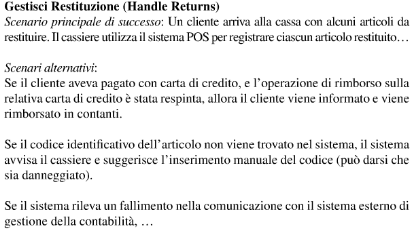
\includegraphics[scale = 0.7]{images/Gestisci restituzione.png}
    \end{center}

}

\dfn{Modello dei Casi d'Uso}{
    Il \newfancyglitter{modello dei Casi d'Uso} è un modello delle funzionalità del sistema. Include un diagramma
    UML dei Casi d'Uso che funge da \newfancyglitter{modello di contesto} del sistema e da \newfancyglitter{indice dei nomi} di Caso d'Uso.

}

\nt{I Casi d'Uso sono utili per rappresentare i requisiti come OOA/D.

I Casi d'Uso definiscono i \newfancyglitter{contratti} (vedi sezione \ref{contratti}) in relazione al comportamento del sistema.}


\subsubsection{L'enfasi è posta sull'utente:}
\begin{itemize}
    \item [$\Rightarrow$] Chi utilizza il sistema?
    \item [$\Rightarrow$] Quali sono i loro Scenari d'Uso tipici?
    \item [$\Rightarrow$] Quali sono i loro obiettivi?
    \item [$\Rightarrow$] \underline{Non} sono caratteristiche del sistema (il "come" si vedrà nella progettazione).
\end{itemize}

\subsection{Attori e tipi di attori}

\dfn{Attore}{
    Un \newfancyglitter{attore} è qualcosa o qualcuno dotato di comportamento.
}

\nt{Il sistema stesso è considerato un attore.}

\subsubsection{Gli attori sono \fancyglitter{ruoli} svolti da persone, organizzazioni, software e macchine:}

\begin{itemize}
    \item [$\Rightarrow$] \fancyglitter{Attore primario}:
    \begin{itemize}
        \item Raggiunge gli obiettivi utente utilizzando il sistema;
        \item Utile per trovare gli obiettivi utente.
    \end{itemize}
    \item [$\Rightarrow$] \fancyglitter{Attore di supporto}:
    \begin{itemize}
        \item Offre un servizio al sistema;
        \item Utile per chiarire le interfacce esterne e i protocolli.
    \end{itemize}
    \item [$\Rightarrow$] \fancyglitter{Fuori scena}:
    \begin{itemize}
        \item Ha un interesse nel comportamento del Caso d'Uso;
        \item Utile per garantire che tutti gli interessi necessari vengano soddisfatti.
    \end{itemize}
\end{itemize}

\subsection{Formato di un Caso d'Uso}

\subsubsection{Un Caso d'Uso può avere tre formati distinti:}

\begin{itemize}
    \item [$\Rightarrow$] \fancyglitter{Breve}: un paragrafo, relativo allo scenario principale di successo. Serve a capire rapidamente l'\newfancyglitter{argomento} e la \newfancyglitter{portata};
    \item [$\Rightarrow$] \fancyglitter{Informale}: più paragrafi, scritti in modo informale, relativi a vari scenari. Si ha un maggior livello di dettaglio;
    \item [$\Rightarrow$] \fancyglitter{Dettagliato}: tutti i passi e le variazioni sono scritti in dettaglio, include \newfancyglitter{pre-condizioni} e \newfancyglitter{garanzie di successo}. Si scrivono a partire da un formato breve o informale.
\end{itemize}

\nt{Durante l'Ideazione il 10\% dei Casi d'Uso è riportato
in formato dettagliato utilizzando appositi \newfancyglitter{template} (e. g. Cockburn).}

\begin{center}
    \begin{tabular}{ || >{\columncolor{mgray}}p{8cm} | >{\columncolor{GreenPastel}}p{8cm} ||}
    \hline\hline
        \rowcolor{lightgray}
    \textbf{Sezione del Caso d'Uso}& \textbf{\textcolor{dkgreen}{Commento}}\\ \hline
    \hline
        Nome del Caso d'Uso & Inizia con un verbo. \\\hline

        Portata & Il sistema che si sta progettando. \\\hline

        Livello & "Obiettivo utente" o "sottofunzione". \\\hline

        Attore primario & Usa direttamente il sistema; gli chiede
        di fornire i suoi servizi per raggiungere un obiettivo. \\\hline

        Parti interessate e interessi & Chiunque abbia un interesse nel comportamento del Caso d'Uso e che cosa desidera. \\\hline

        Pre-condizioni & Stato del sistema prima che il Caso d'Uso inizi. Ciò che vale la pena di dire al lettore. \\\hline

        Garanzia di successo & Che cosa deve essere vero se il Caso d'Uso viene completato con successo. Ciò che vale la pena di dire al lettore. \\\hline  

        Scenario principale di successo & Uno scenario comune di attraversamento del Caso d'Uso, di successo e incondizionato. \\\hline

        Estensioni & Scenari alternativi, di successo o di fallimento. \\\hline

        Requisiti speciali & Requisiti non funzionali correlati. \\\hline

        Elenco delle varianti tecnologiche e dei dati & Varianti dei metodi di I/O e nel formato dei dati. \\\hline

        Frequenza di ripetizione & Quanto spesso si prevede che il Caso d'Uso venga eseguito. \\\hline

        Varie & Altri aspetti. \\\hline

        \hline

    \end{tabular}
\end{center}


\subsection{Come scrivere un Caso d'Uso}

\subsubsection{Sezioni del Caso d'Uso:}

\begin{itemize}
    \item [$\Rightarrow$] \fancyglitter{Portata}: descrive i confini del sistema;
    \item [$\Rightarrow$] \fancyglitter{Livello}: "obiettivo utente" o "sottofunzione";
    \item [$\Rightarrow$] \fancyglitter{Attore finale, attore primario}: l'attore
    finale è l'attore che vuole raggiungere un obiettivo e questo richiede l'esecuzione dei servizi
    del sistema. L'attore primario è l'attore che usa direttamente il sistema. Spesso coincidono;
    \item [$\Rightarrow$] \fancyglitter{Parti interessate}: chiunque abbia un interesse nel comportamento del Caso d'Uso;
    \item [$\Rightarrow$] \fancyglitter{Pre-condizioni}: lo stato del sistema prima che il Caso d'Uso inizi. Non vengono verificate all'interno del Caso d'Uso;
    \item [$\Rightarrow$] \fancyglitter{Garanzie di successo} (post-condizioni): ciò che deve essere vero se il Caso d'Uso viene completato con successo.
\end{itemize}

\subsubsection{Caratteristiche:}

\begin{itemize}
    \item [$\Rightarrow$] Lo scenario principale viene anche chiamato "\fancyglitter{percorso felice}", "flusso
    di base" o "flusso tipico";
    \item [$\Rightarrow$] Lo scenario principale è costituito da una sequenza di passi, che può contenere passi da ripetere, ma che non comprende nessuna diramazione\footnote{\underline{Non} è un algoritmo.};
    \item [$\Rightarrow$] La gestione del comportamento condizionale e delle alternative viene descritta nelle "\fancyglitter{estensioni}".
\end{itemize}

\subsubsection{I passi possono essere di 3 tipi:}

\begin{itemize}
    \item [$\Rightarrow$] \fancyglitter{Un'interazione tra attori}: 
    \begin{itemize}
        \item Un attore chiede qualcosa al sistema o inserisce dei dati;
        \item Il sistema interagisce con l'attore, rispondendo o comunicando dei dati;
        \item Il sistema interagisce con altri sistemi.
    \end{itemize}
    \item [$\Rightarrow$] \fancyglitter{Un cambiamento di stato da parte del sistema};
    \item [$\Rightarrow$] \fancyglitter{Una validazione}: normalmente fatta dal sistema.
\end{itemize}

\nt{Il primo passo indica l'evento \textit{trigger} che scatena l'esecuzione dello scenario.}

\subsubsection{Estensioni:}

\begin{itemize}
    \item [$\Rightarrow$] Descrivono tutti gli altri scenari;
    \item [$\Rightarrow$] Sono descritte per differenza rispetto allo scenario principale;
    \item [$\Rightarrow$] Vengono indicate con riferimento a un passo dello scenario principale;
    \item [$\Rightarrow$] Sono composte da:
    \begin{itemize}
        \item \fancyglitter{Condizione}: che scatena l'estensione;
        \item \fancyglitter{Gestione}: come viene gestita l'estensione. Può essere di un unico passo o di più passi.
    \end{itemize}
\end{itemize}

\nt{Le condizioni vanno scritte, se possibile, come qualcosa che può essere rilevato da un attore.}

\cor{Utilizzo delle estensioni}{
    \begin{itemize}
        \item [$\Rightarrow$] L'attore vuole che l'esecuzione principale del Caso d'Uso proceda in modo diverso da quanto previsto nel percorso felice;
        \item [$\Rightarrow$] Il Caso d'Uso deve procedere diversamente da quanto previsto ed è il sistema che se ne accorge (durante un'azione o una validazione);
        \item [$\Rightarrow$] Un passo dello scenario principale descrive un'azione generica o astratta, mentre le estensioni
        descrivono azioni specifiche o concrete.
    \end{itemize}
}
\pagebreak
\subsubsection{Notazione:}

\begin{itemize}
    \item [$\Rightarrow$] Si può utilizzare il formato a due colonne. Questo enfatizza
    la \fancyglitter{conversazione} tra gli attori e il sistema\footnote{È il formato scelto per il laboratorio del corso.}.
    \begin{figure}[!h]
        \centering
        \subfloat[Rappresentazione come conversazione]{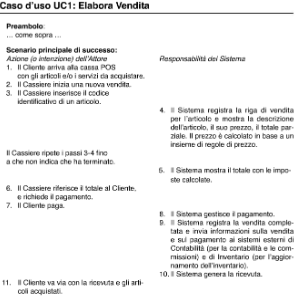
\includegraphics[scale = 0.65]{images/Notazione.png}} 
        \subfloat[Relativa tabella]{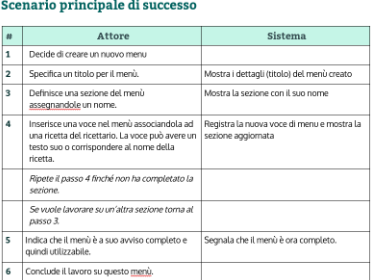
\includegraphics[scale = 0.65]{images/Notazione2.png}}
    \end{figure}
    \item [$\Rightarrow$] Le estensioni vanno indicate con riferimento al passo dello scenario principale.
\begin{figure}[!h]
    \centering
    \subfloat[Estensione del punto 1]{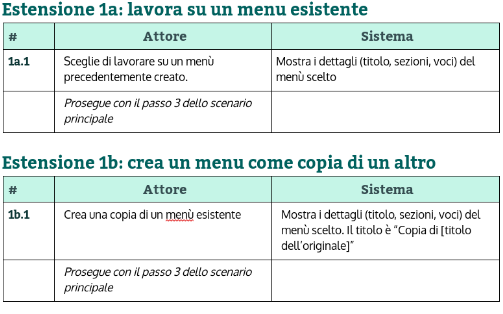
\includegraphics[scale = 0.4]{images/Estensione1.png}} 
    \subfloat[Estensione del punto 3]{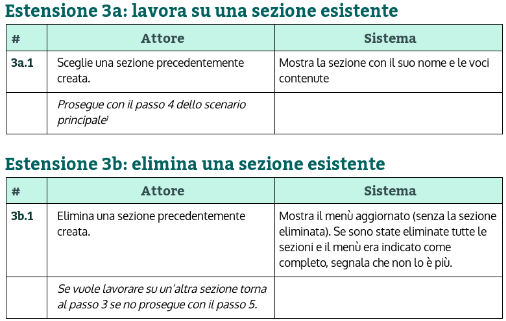
\includegraphics[scale = 0.4]{images/Estensione2.png}}
\end{figure}
\item [$\Rightarrow$] Ci possono essere alternative che possono occorrere in più passi.
\begin{figure}[!h]
    \centering
    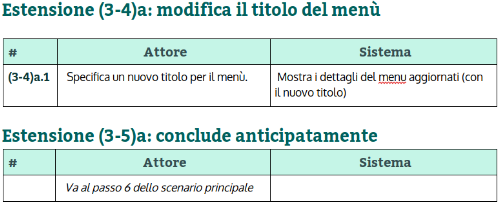
\includegraphics[scale = 0.55]{images/Estensione3.png}
\end{figure}
\end{itemize}

\ex{Passi ed estensioni}{
    \begin{center}
        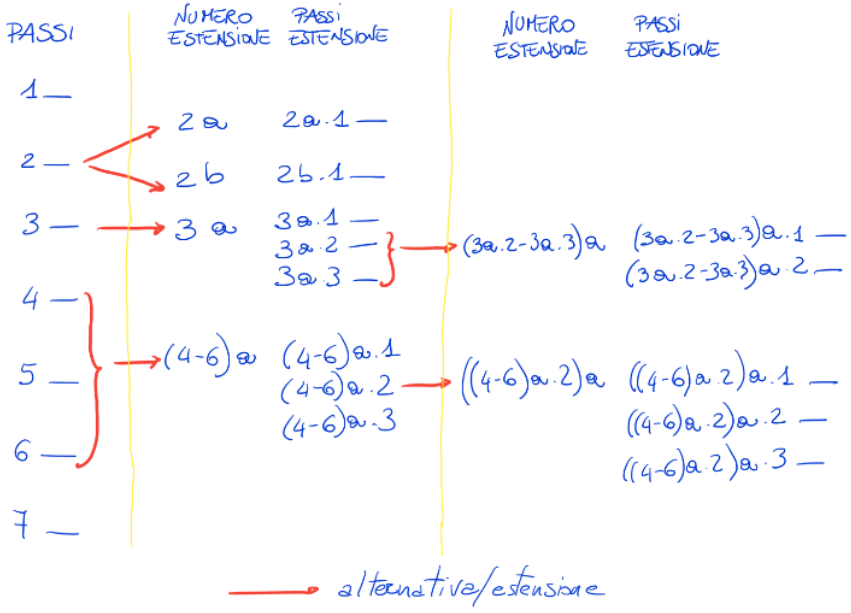
\includegraphics[scale = 0.4]{images/Passi ed estensioni.png}
    \end{center}
}

\nt{Lo stile deve essere \newfancyglitter{essenziale} e \newfancyglitter{coinciso}. Si ignora l'interfaccia utente, ci si concentra sull'Obiettivo Utente.}

\dfn{Stile essenziale}{
    La narrativa è espressa a livello di \newfancyglitter{intenzioni} e 
    \newfancyglitter{responsabilità}, non con riferimento ad azioni concrete.
    Le intenzioni e le responsabilità devono rimanere indipendenti dai dettagli tecnologici e dagli attori.
}

\ex{Stile}{
    \begin{itemize}
        \item [\textcolor{dkgreen}{\checkmark}] L'Amministratore si identifica.
        \item [\textcolor{dkgreen}{\checkmark}] Il Sistema autentica l'identità.
        \item [\textcolor{red}{\XSolidBrush}] L'Amministratore inserisce ID e password nella finestra di dialogo.
        \item [\textcolor{red}{\XSolidBrush}] Il sistema autentica l'Amministratore.
        \item [\textcolor{red}{\XSolidBrush}] Il sistema visualizza la finestra "edit users".
    \end{itemize}
}

\clm{}{}{Durante l'analisi dei requisiti bisogna specificare il comportamento
esterno del Sistema, considerato a "scatola nera". Non bisogna prendere decisioni
sul "come".

\begin{itemize}
    \item [\textcolor{red}{\XSolidBrush}] Il Sistema memorizza la vendita in una base di dati.
    \item [\textcolor{red}{\XSolidBrush}] Il Sistema esegue un'istruzione SQL INSERT per la vendita.
\end{itemize}
}

\subsection{Trovare i Casi d'Uso}

\begin{enumerate}
    \item Scegliere i confini del Sistema;
    \item Identificare gli attori primari;
    \item Identificare gli obiettivi di ciascun attore primario;
    \item Definire i Casi d'Uso che soddisfano gli obiettivi degli utenti.
\end{enumerate}

\ex{Identificare gli attori primari}{
    \begin{center}
        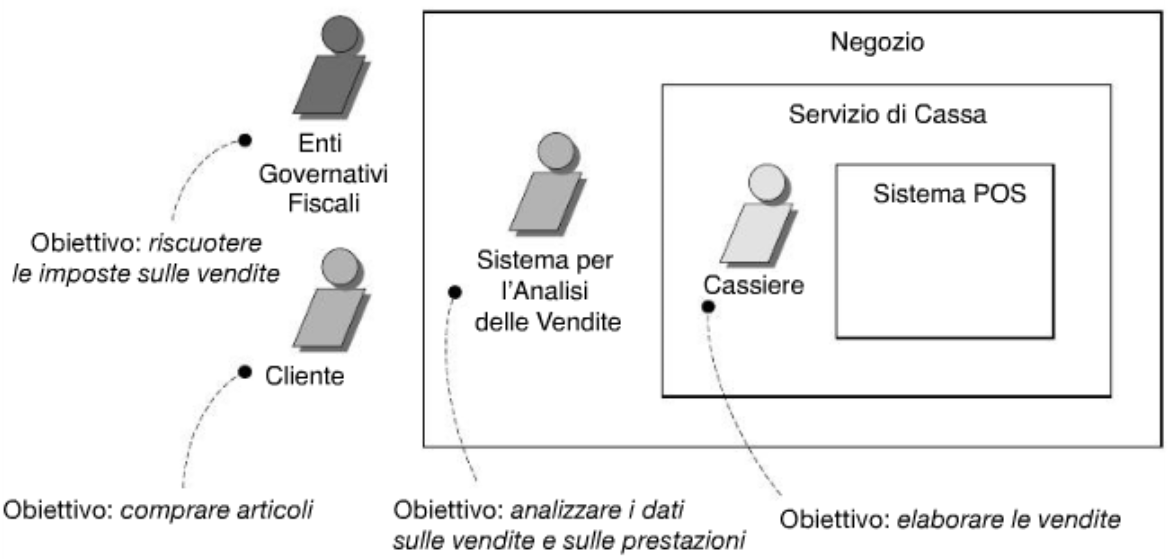
\includegraphics[scale = 0.3]{images/Identificare gli attori primari.png}
        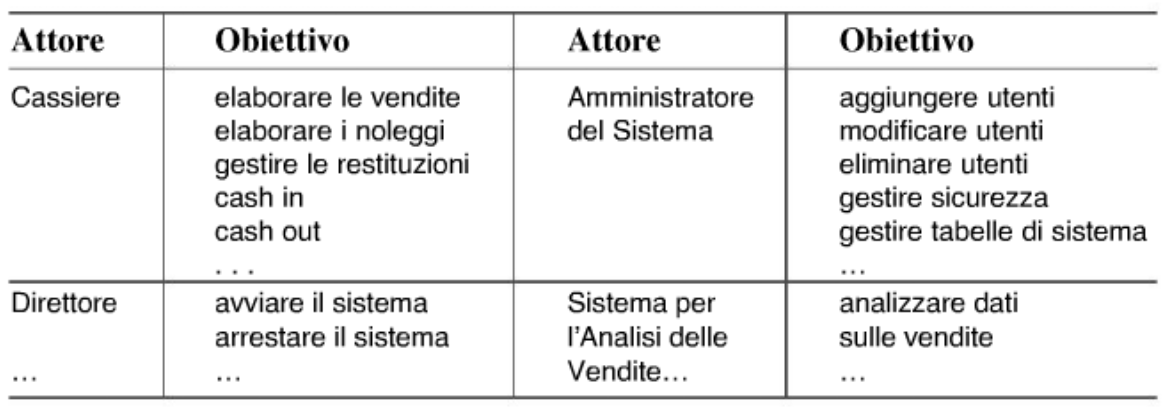
\includegraphics[scale = 0.3]{images/Identificare gli attori 2.png}
    \end{center}

}

\qs{}{Qual è un livello utile per esprimere i Casi d'Uso nell'analisi dei requisiti di un'applicazione software?}
\begin{itemize}
    \item [$\Rightarrow$] Il test del \fancyglitter{capo}: il capo sarà felice?
    \item [$\Rightarrow$] Il test \fancyglitter{EBP} (Elementary Business Process): un processo di Business è un'attività che aggiunge un valore;
    \item [$\Rightarrow$] Il test della \fancyglitter{dimensione}: un Caso d'Uso raramente richiede una singola azione o passo. Normalmente, nella forma dettagliata, richiede dalle 3 alle 10 pagine.
\end{itemize}

\ex{Verificare l'utilità dei Casi d'Uso}{
    \begin{itemize}
        \item \textcolor{red}{\XSolidBrush} Negoziare un contratto con un fornitore.
        \begin{itemize}
            \item [$\Rightarrow$] Troppo grande.

        \end{itemize}
        \item \textcolor{dkgreen}{\checkmark} Gestire una restituzione.
        \begin{itemize}
            \item [$\Rightarrow$] D'accordo con il capo, simile a EBP, dimensioni adeguate.
        \end{itemize}
        \item \textcolor{red}{\XSolidBrush} Effetture il login.
        \begin{itemize}
            \item [$\Rightarrow$] Il capo non è contento se ci si limita a fare solo quello tutta la giornata.
        \end{itemize}
        \item \textcolor{red}{\XSolidBrush} Spostare una pedina sul tabellone da gioco.
        \begin{itemize}
            \item [$\Rightarrow$] Passo singolo, non supera il test della dimensione.
        \end{itemize}
    \end{itemize}
}

\subsection{Livello dei Casi d'Uso}

\dfn{Livello di obiettivo utente}{
    Nell'analisi dei requisiti è utile concentrarsi sui casi utente EBP.
}

\dfn{Livello di sotto-funzione}{
    Rappresenta una funzionalità nell'uso del sistema.
    Utile per mettere a fattor comune sequenze di passi condivise da più Casi
    d'Uso, evitando duplicazione di testo.
}

\ex{Diagramma dei Casi d'Uso (UCD)}{
    \begin{center}
        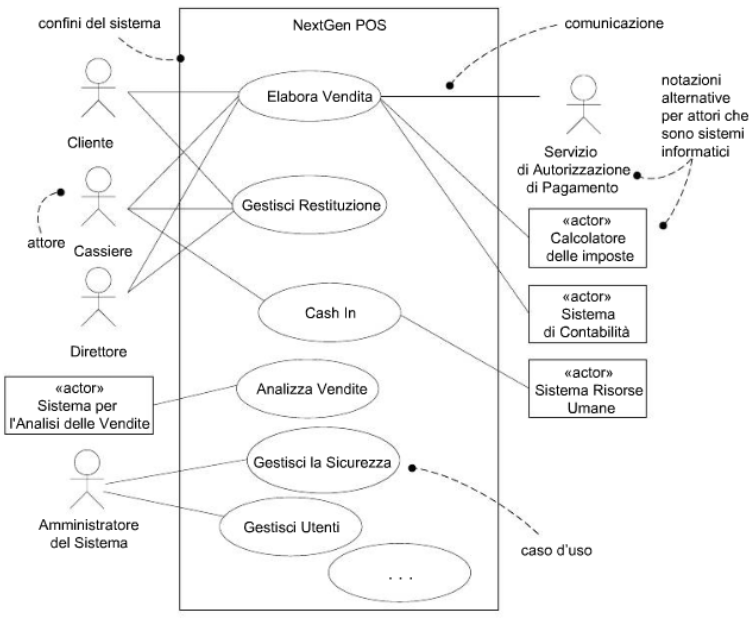
\includegraphics[scale = 0.5]{images/UCD.png}
    \end{center}

}
\section{Elaborazione}

\dfn{Elaborazione}{
    L'elaborazione è la serie iniziale di iterazioni durante le quali il team
    esegue un'indagine seria, implementa il nucleo dell'architettura,
    chiarisce la maggior parte dei requisiti e affronta le problematiche
    più rischiose.
}

\nt{Durante questa fase vengono creati prototipi "usa e getta" ma codice
e progettazione sono parti di qualità-produzione del sistema finale.}

\subsection{Pianificazione dell'iterazione successiva}

I requisiti e le iterazioni sono organizzate in base a:

\begin{itemize}
    \item [$\Rightarrow$] \fancyglitter{Rischio}: tecnico, incertezza dello sforzo, usabilità;
    \item [$\Rightarrow$] \fancyglitter{Copertura}: le iterazioni iniziali devono coprire tutte le parti principali del sistema;
    \item [$\Rightarrow$] \fancyglitter{Criticità}: le funzioni che il cliente ritiene più importanti.
\end{itemize}

\clm{}{}{La classifica viene stilata prima dell'iterazione 1, poi prima dell'iterazione 2 e così via. La lista non è definitiva.

\begin{center}
    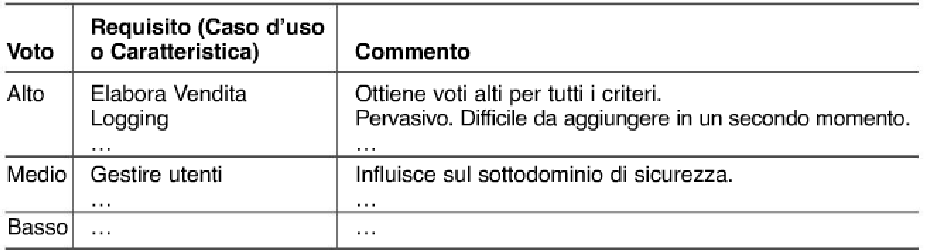
\includegraphics[scale=0.48]{images/Classifica.png}
\end{center}
}

\dfn{Iterazione 1}{
    Nell'iterazione 1 si implementa un sottoinsieme dei requisiti o dei Casi d'Uso completi.
}

\subsection{Artefatti dell'Elaborazione}

\begin{center}
    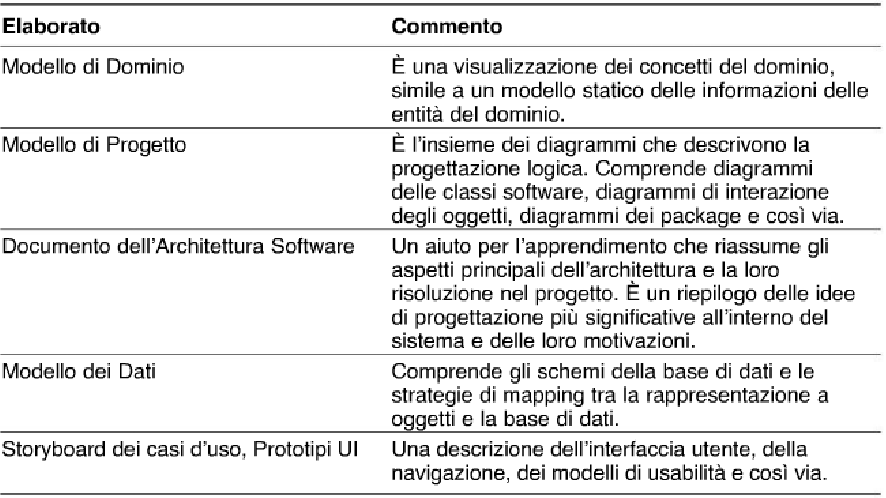
\includegraphics[scale=0.5]{images/Artefatti elaborazione.png}
\end{center}

\begin{center}
    
\end{center}

\section{Modello di Dominio}

\dfn{Modello di Dominio}{
    Il \newfancyglitter{Modello di Dominio} è una rappresentazione visuale
    delle classi concettuali (oggetti del dominio). Include:
    \begin{itemize}
        \item [\textcolor{green}{\checkmark}] \newfancyglitter{Oggetti} di dominio.
        \item [\textcolor{green}{\checkmark}] \newfancyglitter{Associazioni} tra classi concettuali.
        \item [\textcolor{green}{\checkmark}] \newfancyglitter{Attributi} di classi concettuali.
        \item [\textcolor{red}{\XSolidBrush}] \newfancyglitter{Operazioni}.
    \end{itemize}
}

\nt{Non è un modello di dati.}

\ex{Modello di dominio}{
    \begin{center}
        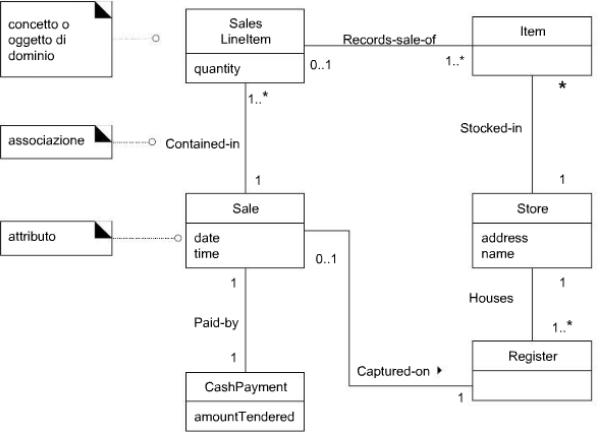
\includegraphics[scale=0.5]{images/Modello di dominio.png}
    \end{center}

}

\subsection{Classi concettuali}

\dfn{Classi concettuali}{
    Una \newfancyglitter{classe concettuale} rappresenta un concetto
    del mondo reale o del dominio di interesse di un sistema che si sta modellando.

    \begin{itemize}
        \item [$\Rightarrow$] Il \newfancyglitter{simbolo} è una parola 
        o un'immagine usata per rappresentare la classe concettuale;
        \item [$\Rightarrow$] L'\newfancyglitter{intensione} è la definizione della classe concettuale;
        \item [$\Rightarrow$] L'\newfancyglitter{estensione} è l'insieme di oggetti che la classe concettuale rappresenta.
    \end{itemize}
}
\pagebreak
\cor{Associazioni}{
    Un'associazione è una relazione tra istanze di classi
    che indica una connessione significativa e interessante.
}

\ex{Associazione}{
    \begin{center}
        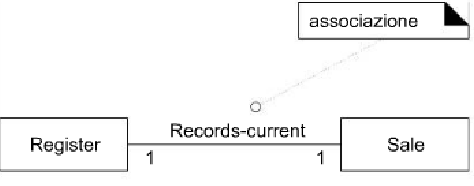
\includegraphics[scale=0.5]{images/Associazione.png}
    \end{center}


}

\cor{Attributi}{
    Un attributo è un valore logico degli oggetti di una classe.
}

\ex{Attributo}{
    \begin{center}
        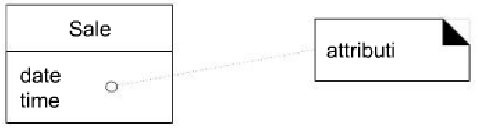
\includegraphics[scale=0.5]{images/Attributo.png}
    \end{center}
}

\subsubsection{Riduzione del "gap di rappresentazione":}

\begin{itemize}
    \item [$\Rightarrow$] \fancyglitter{Comprendere} il dominio del sistema da realizzare e il suo vocabolario;
    \item [$\Rightarrow$] \fancyglitter{Definire} un \fancyglitter{linguaggio comune} che abiliti la comunicazione tra le diverse parti;
    \item [$\Rightarrow$] Come \fancyglitter{fonte di ispirazione} per la progettazione dello strato di dominio.
\end{itemize}

\qs{}{Come creare un Modello di Dominio}

\begin{itemize}
    \item [$\Rightarrow$] Trovare le classi concettuali;
    \item [$\Rightarrow$] Disegnarle come classi in UML;
    \item [$\Rightarrow$] Aggiungere le associazioni;
    \item [$\Rightarrow$] Aggiungere gli attributi.
\end{itemize}

\subsection{Trovare le classi concettuali}

\begin{itemize}
    \item [$\Rightarrow$] Riuso-modifica di modelli esistenti (pattern);
    \item [$\Rightarrow$] Utilizzo di elenchi di categorie;
    \item [$\Rightarrow$] Analisi linguistica delle descrizioni testuali di un dominio. 
    Si utilizano i Casi d'Uso dettagliati.
\end{itemize}

\dfn{Classi Descrizione}{
    Una \newfancyglitter{classe descrizione} contiene informazioni
    che descrivono qualcos'altro. È utile avere un'associazione
    che collega la classe descrizione alla classe descritta\footnote{Pattern Item-Descriptor.}.
}

\ex{Classe descrizione}{
    \begin{center}
        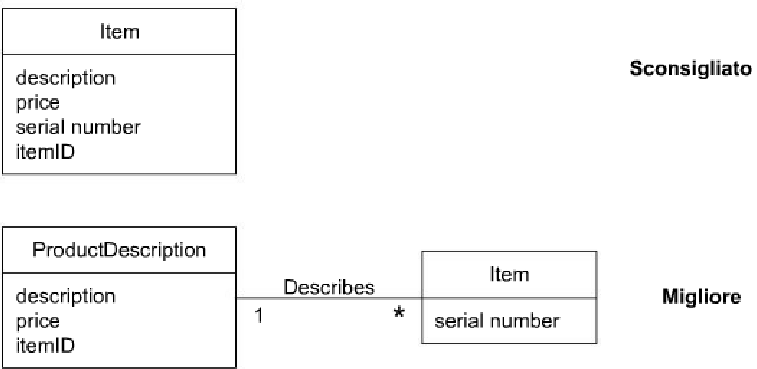
\includegraphics[scale=0.5]{images/Classe descrizione.png}
    \end{center}
}

\subsection{Associazioni}

\subsubsection{È utile includere:}

\begin{itemize}
    \item [$\Rightarrow$] Associazioni la cui conoscenza della relazione deve
    essere mantenuta dal sistema;
    \item [$\Rightarrow$] Associazioni derivate dall'elenco di associazioni comuni.
\end{itemize}

\nt{Un'associazione è per natura \fancyglitter{bidirezionale}.}

\begin{center}
    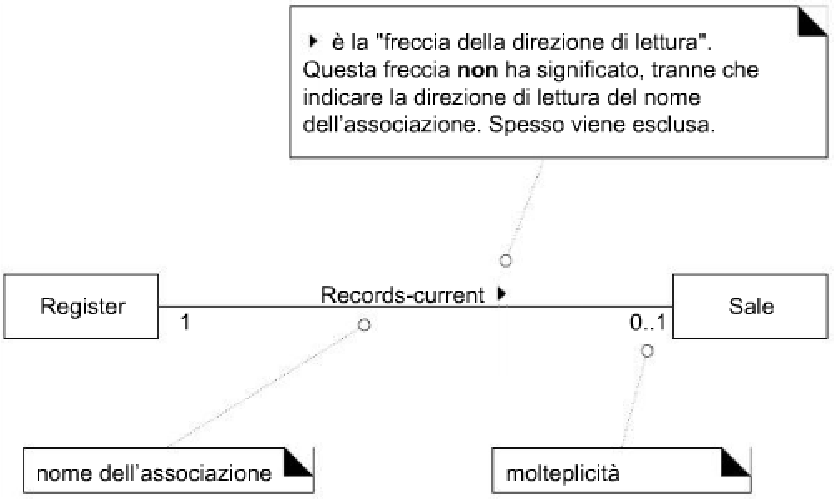
\includegraphics[scale=0.4]{images/Associazione2.png}
\end{center}

\subsubsection{Caratteristiche delle associazioni:}

\begin{itemize}
    \item [$\Rightarrow$] \fancyglitter{Nome significativo}: NomeClasse-FraseVerbale-NomeClasse;
    \item [$\Rightarrow$] \fancyglitter{Molteplicità e direzione di lettura}.
\end{itemize}

\dfn{Ruoli}{
    Un \newfancyglitter{ruolo} è l'estremità di un'associazione. I ruoli possono avere:
    \begin{itemize}
        \item [$\Rightarrow$] \newfancyglitter{Nome};
        \item [$\Rightarrow$] \newfancyglitter{Molteplicità};
        \item [$\Rightarrow$] \newfancyglitter{Navigabilità}.
    \end{itemize}


}

\cor{Molteplicità}{
    La molteplicità di un ruolo definisce quante istanze di una classe possono
    essere associate a un'istanza dell'altra classe.
}

\ex{Molteplicità}{
    \begin{center}
        \includegraphics[scale=0.5]{images/Molteplicità.png}
    \end{center}
}

\subsection{Composizione}

\dfn{Composizione}{
    La \newfancyglitter{composizione}, o aggregazione composta,
    è un tipo forte di aggregazione intero-parte:
    \begin{itemize}
        \item [$\Rightarrow$] Ciascuna istanza della parte appartiene a una sola istanza del composto alla volta;
        \item [$\Rightarrow$] La parte non può esistere senza il composto;
        \item [$\Rightarrow$] La vita delle parti è limitata a quella del composto.
    \end{itemize}
}

\subsection{Attributi}

\subsubsection{Caratteristiche degli attributi:}

\begin{itemize}
    \item [$\Rightarrow$] \fancyglitter{Origine}: derivati/non derivati;
    \item [$\Rightarrow$] \fancyglitter{Tipo di dato}: vincolo sui valori del dominio.
\end{itemize}

\begin{center}
    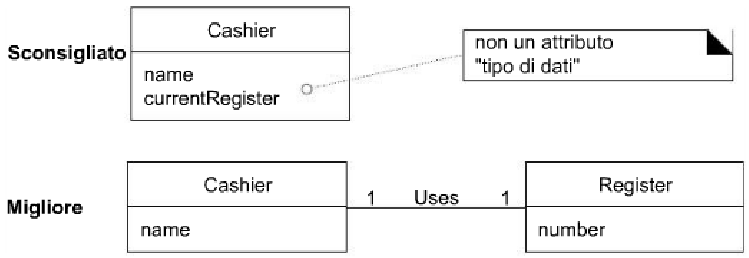
\includegraphics[scale=0.5]{images/Attributi2.png}
\end{center}

\nt{Se non si pensa a un concetto come a un numero, un testo o un
valore allora probabilmente è una classe, non un attributo.}

\begin{center}
    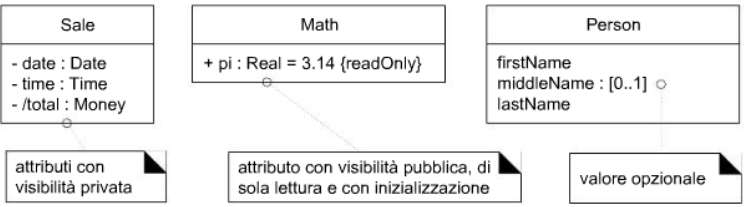
\includegraphics[scale=0.5]{images/Notazione attributi.png}
\end{center}


\subsection{Verifiche del modello}

\begin{itemize}
    \item [$\Rightarrow$] Verificare le classi concettuali introdotte:
    \begin{itemize}
        \item Alternativa classe classe-attributo attributo;
        \item Classi descrizione.
    \end{itemize}
    \item [$\Rightarrow$] Verificare le associazioni:
    \begin{itemize}
        \item Indipendenza delle associazioni diverse relative alle stesse classi.
    \end{itemize}
    \item [$\Rightarrow$] Verificare gli attributi:
    \begin{itemize}
        \item Non intrododurre attributi per riferirsi ad altre classi (chiavi esterne).
    \end{itemize}
\end{itemize}

\ex{Modello di Dominio (parziale)}{
    \begin{center}
        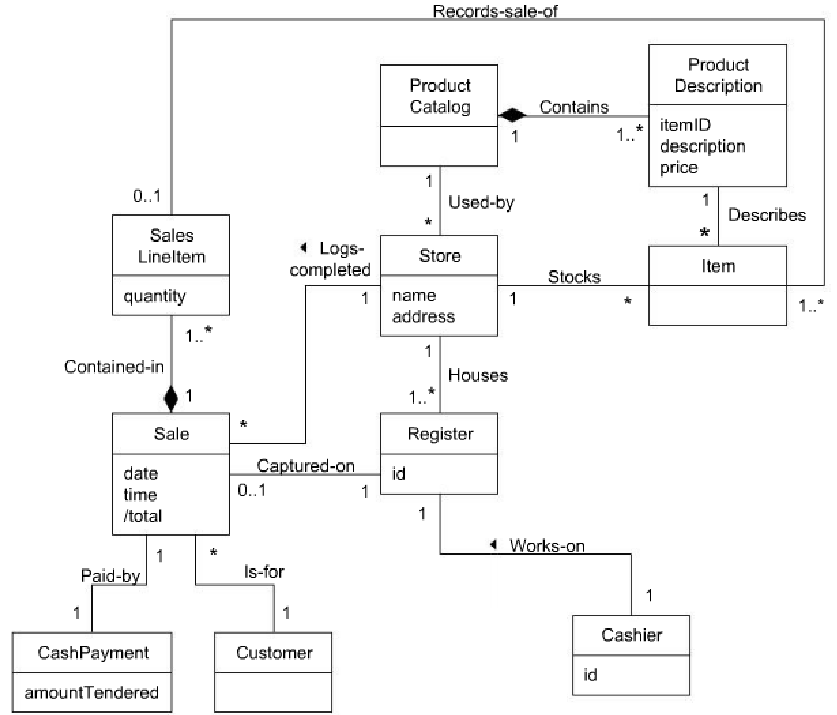
\includegraphics[scale=0.5]{images/Modello di Dominio.png}
    \end{center}

}
\dfn{Generalizzazione}{
    La \newfancyglitter{generalizzazione} è un'astrazione basata sull'identificazione
    di caratteristiche comuni tra concetti, che porta a definire un concetto più generale 
    (superclasse) e concetti più specifici (sottoclassi). Vale il principio di sostituibilità.
}

\ex{Generalizzazione}{
    \begin{center}
        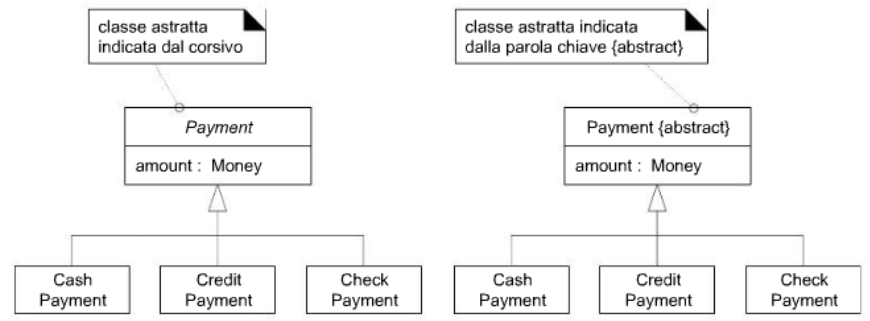
\includegraphics[scale=0.45]{images/Generalizzazione.png}
    \end{center}


}

\section{Diagrammi di sequenza del sistema (SSD)}

\dfn{SSD}{
    Il \newfancyglitter{Diagramma di Sequenza del Sistema} è un elaborato
    della disciplina dei requisitiche illustra eventi di input e di output
    relativi ai sistemi in discussione.

    È una figura che mostra, per un particolare Caso d'Uso, gli eventi
    generati dagli attori esterni al sistema, il loro ordine e gli eventi inter-sistema.
}

\nt{Di solito si usa un SSD per ogni Caso d'Uso.}

\cor{Eventi}{
    Durante un'interazione con il sistema software, un attore genera degli 
    eventi di sistema, che costituiscono un input
    per il sistema, di solito per richiedere l'esecuzione di
    alcune operazioni di sistema.

    \begin{itemize}
        \item [$\Rightarrow$] Le operazioni di sistema sono operazioni che il sistema
        deve definire proprio per gestire tali eventi;
        \item [$\Rightarrow$] Un evento deve essere degno di nota;
        \item [$\Rightarrow$] Un evento di sistema è un evento esterno al sistema generato
        da un attore per interagire con il sistema.
    \end{itemize}
}

\subsubsection{Un sistema reagisce a:}

\begin{itemize}
    \item [$\Rightarrow$] \fancyglitter{Eventi esterni}: generati da attori umani o sistemi informatici;
    \item [$\Rightarrow$] \fancyglitter{Eventi temporali};
    \item [$\Rightarrow$] \fancyglitter{Guasti o eccezioni}.
\end{itemize}


\nt{Il software deve essere progettato per gestire questi eventi.}

\ex{SSD}{
    \begin{center}
        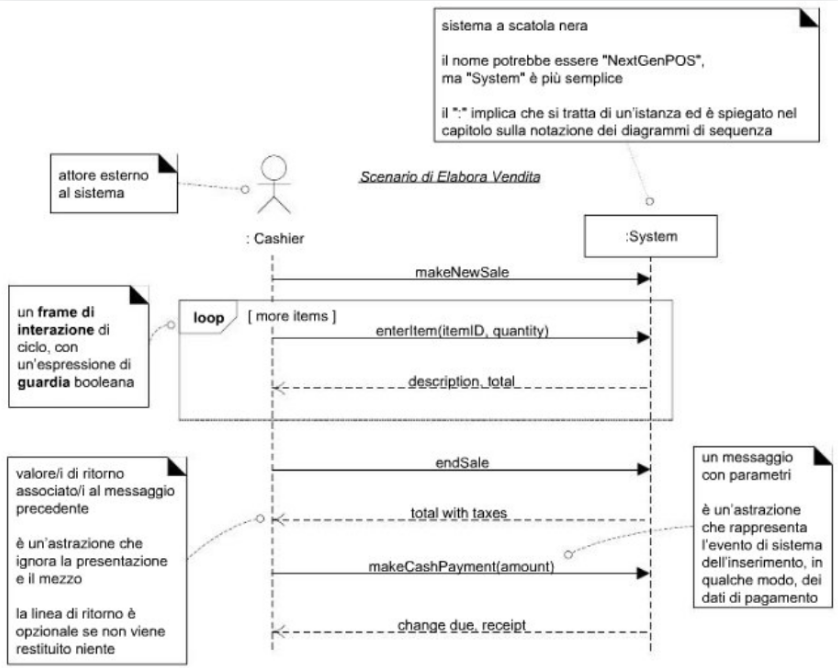
\includegraphics[scale=0.35]{images/SSD.png}
    \end{center}
\pagebreak
    \begin{itemize}
        \item [$\Rightarrow$] \textit{makeNewSale}: il cassiere inizia una nuova vendita;
        \item [$\Rightarrow$] \textit{enterItem}: il cassiere inserisce il codice identificativo di un articolo;
        \item [$\Rightarrow$] \textit{endSale}: il cassiere indica di aver terminato l'inserimento degli articoli acquistati;
        \item [$\Rightarrow$] \textit{makeCashPayment}: il cassiere indica che il cliente sta pagando in contanti e inserisce l'importo offerto dal cliente. 
    \end{itemize}


}

\subsubsection{Un SSD mostra:}

\begin{itemize}
    \item [$\Rightarrow$] L'attore primario del Caso d'Uso;
    \item [$\Rightarrow$] Il sistema in discussione;
    \item [$\Rightarrow$] I passi che rappresentano le interazioni tra il sistema e l'attore.
\end{itemize}

\nt{Le interazioni sono mostrate come messaggi con parametri.}

\subsection{Notazione}

\subsubsection{\fancyglitter{Semplice diagramma di sequenza:}}

\begin{center}
    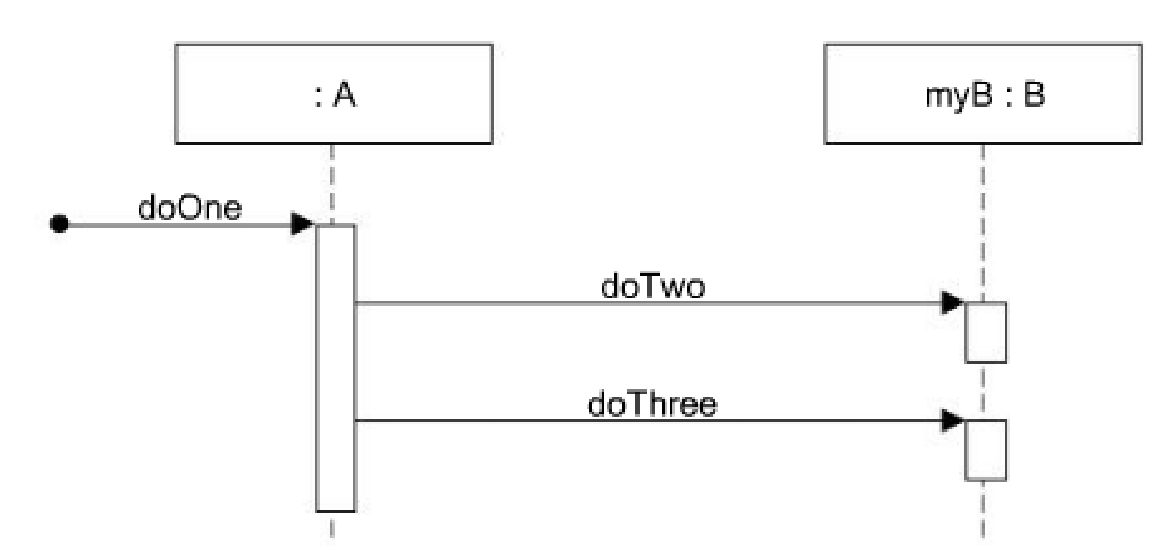
\includegraphics[scale=0.33]{images/Notazione SSD.png}
\end{center}

\subsubsection{\fancyglitter{Mostrare il risultato di ritorno:}}

\begin{center}
    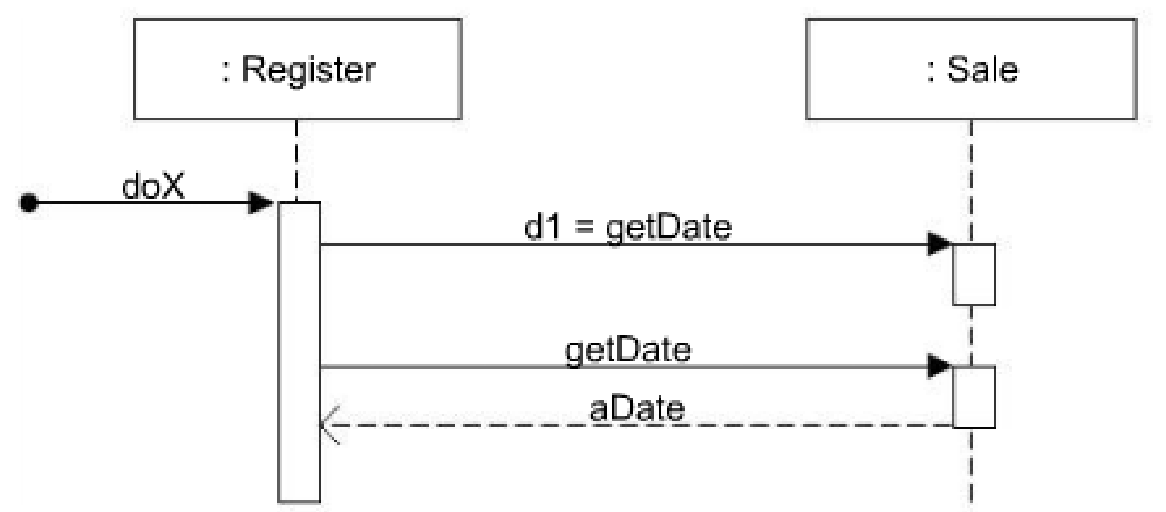
\includegraphics[scale=0.33]{images/Notazione SSD2.png}
\end{center}

\subsubsection{\fancyglitter{Frame di UML:}}

\begin{center}
    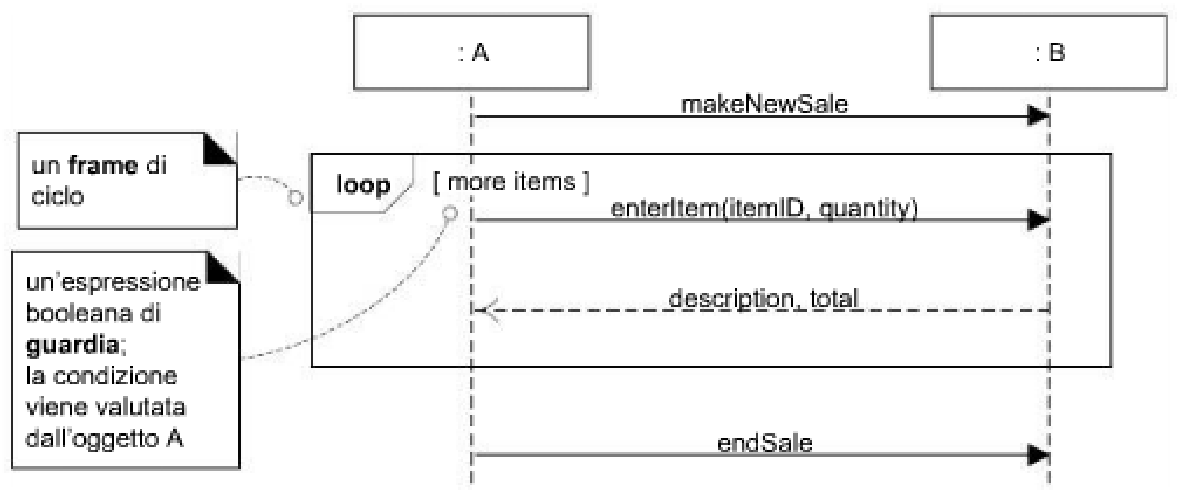
\includegraphics[scale=0.33]{images/Notazione SSD3.png}
\end{center}

\subsubsection{\fancyglitter{Operatori comuni per i frame UML:}}

\begin{center}
    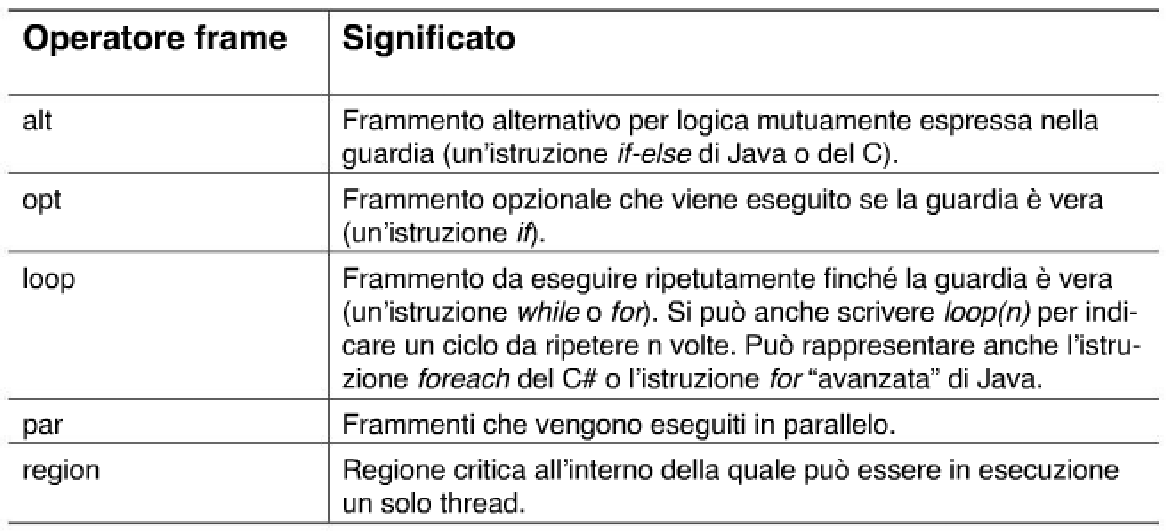
\includegraphics[scale=0.33]{images/Notazione SSD4.png}
\end{center}

\subsubsection{\fancyglitter{Annidamento di frame:}}

\begin{center}
    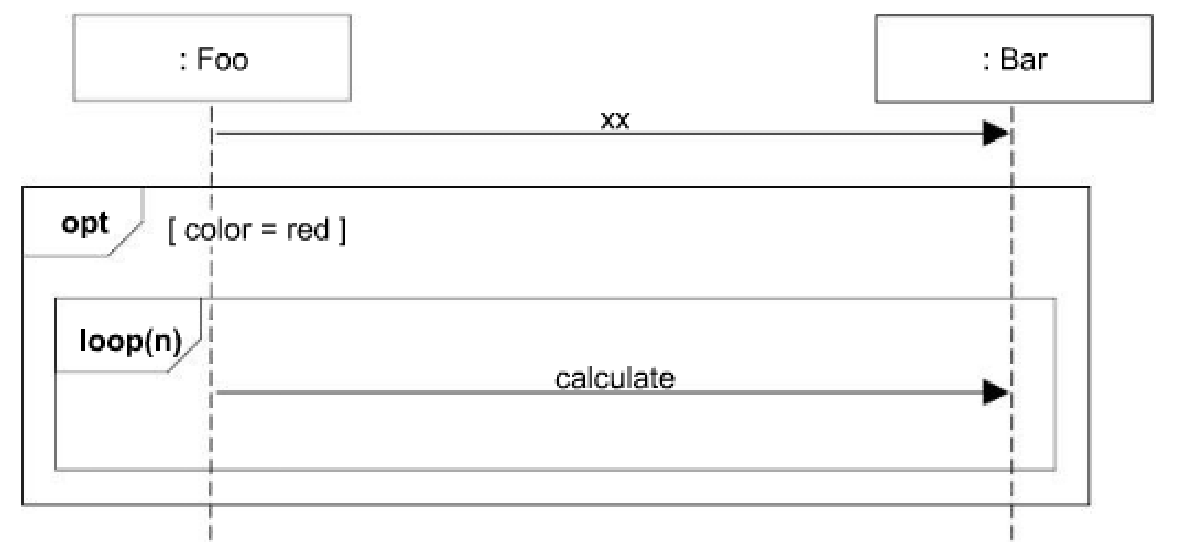
\includegraphics[scale=0.33]{images/Notazione SSD5.png}
\end{center}

\section{Contratti}
\label{contratti}

\subsection{Pre-condizioni e Post-condizioni}

\dfn{I contratti delle operazioni}{
    I contratti usano \newfancyglitter{pre-condizioni} e \newfancyglitter{post-condizioni} per descrivere nel
    dettaglio i cambiamenti agli oggetti in un Modello di Dominio.

    \paragraph{Punto di vista:}
    \begin{itemize}
        \item [\textcolor{dkgreen}{\checkmark}] Concettuale.
        \item [\textcolor{red}{\XSolidBrush}] Implementativo.
    \end{itemize}
}

\nt{Possono essere considerati parte del Modello dei Casi d'Uso, ma non sono
menzionati esplicitamente in UP.}

\ex{Contratto}{

    \begin{center}
        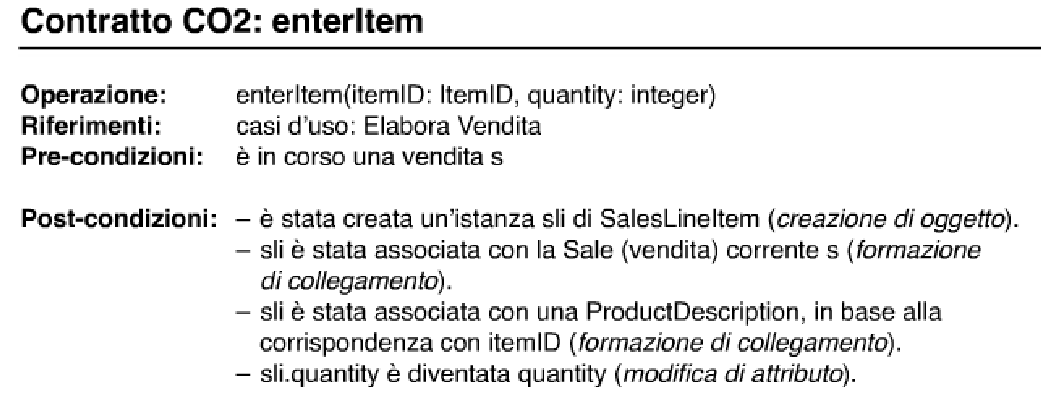
\includegraphics[scale=0.35]{images/Contratto.png}
    \end{center}
}

\subsubsection{Template di un contratto:}

\begin{itemize}
    \item [$\Rightarrow$] \fancyglitter{Operazione}: Nome e parametri dell'operazione;
    \item [$\Rightarrow$] \fancyglitter{Riferimenti}: Casi d'Uso in cui può verificarsi l'operazione;
    \item [$\Rightarrow$] \fancyglitter{Pre-condizioni}: Stato del sistema prima dell'operazione. Sono ipotesi non banali;
    \item [$\Rightarrow$] \fancyglitter{Post-condizioni}: Stato del sistema dopo l'operazione. 
\end{itemize}

\dfn{Post-condizioni}{
    Le \newfancyglitter{post-condizioni} descrivono i cambiamenti nello stato degli oggetti
    del Modello di Dominio. I cambiamenti comprendono:
    
    \begin{itemize}
        \item [$\Rightarrow$] Oggetti creati;
        \item [$\Rightarrow$] Collegamenti formati;
        \item [$\Rightarrow$] Collegamenti rotti;
        \item [$\Rightarrow$] Attributi modificati.
    \end{itemize}

}

\nt{Le post-condizioni sono osservazioni al termine dell'operazione.
Ci si concentra sul "cosa", ma non sul "come".}

\dfn{Pre-condizioni}{
    Le \newfancyglitter{pre-condizioni} sono ipotesi sullo stato del sistema
    prima dell'operazione. Sono condizioni che devono essere vere
    prima che l'operazione possa essere eseguita.
}

\nt{Le pre-condizioni sono una descrizione sintetica sullo stato
di avanzamento del Caso d'Uso.}

\subsection{Scrivere contratti}

\subsubsection{Si procede così:}

\begin{enumerate}
    \item Si identificano le operazioni dagli SSD;
    \item Si crea un contratto per le operazioni complesse
    o i cui effetti sono sottili (non chiari dai Casi d'Uso);
    \item Si scrivono le pre-condizioni e le post-condizioni:
    \begin{itemize}
        \item [$\Rightarrow$] creazione o cancellazione di oggetti;
        \item [$\Rightarrow$] formazione o rottura di collegamenti;
        \item [$\Rightarrow$] modifica di attributi.
    \end{itemize}
\end{enumerate}

\nt{Ogni operazione può avere una componente di:

\begin{itemize}
    \item [$\Rightarrow$] \fancyglitter{Trasformazione}: modifica lo stato del sistema;
    \item [$\Rightarrow$] \fancyglitter{Interrogazione}: non modifica lo stato del sistema, vengono restituiti valori.
\end{itemize}

Un'operazione ha post-condizioni solo se è di trasformazione, mentre
non le ha se è di interrogazione.
}

\qs{}{Bisogna scrivere un contratto per ogni evento di sistema trovato nel SSD?}

\paragraph{Risposta:} Non è necessario, si considerano solo quelli più complessi.
\paragraph{}
\qs{}{Se si scoprono nuove classi, attributi, si possono aggiungere nel modello di dominio?}

\paragraph{Risposta:} Sì, UP è incrementale.
\paragraph{}
\qs{}{Le post-condizioni devono essere in ogni momento le pi`u complete possibili?}

\paragraph{Risposta:} Non è necessario.
